\documentclass[a4paper, fleqn]{article}
\usepackage{header}
\pgfplotsset{compat=1.17}
\usepgfplotslibrary{fillbetween}
\usetikzlibrary{patterns}

\title{Семинарский лист 2.5}
\author{
    % Александр Богданов   \\ \href{https://t.me/SphericalPotatoInVacuum}{Telegram} \and
    % Алиса Вернигор       \\ \href{https://t.me/allisyonok}{Telegram} \and
    Анастасия Григорьева \\ \href{https://t.me/weifoll}{Telegram} \and
    % Василий Шныпко       \\ \href{https://t.me/yourvash}{Telegram} \and
    % Данил Казанцев       \\ \href{https://t.me/vserosbuybuy}{Telegram} \and
    Денис Козлов         \\ \href{https://t.me/DKozl50}{Telegram} \and
    Елизавета Орешонок   \\ \href{https://t.me/eaoresh}{Telegram} \and
    Ира Голобородько     \\ \href{https://t.me/Ira4kgl}{Telegram}
    % Иван Пешехонов       \\ \href{https://t.me/JohanDDC}{Telegram} \and
    % Иван Добросовестнов  \\ \href{https://t.me/ivankot13}{Telegram} \and
    % Настя Городилова     \\ \href{https://t.me/nastygorodi}{Telegram} \and
    % Никита Насонков      \\ \href{https://t.me/nnv_nick}{Telegram} \and
    % Сергей Лоптев        \\ \href{https://t.me/beast_sl}{Telegram}
}

\date{Версия от {\ddmmyyyydate\today} \currenttime}

\begin{document}
    \maketitle
    
    \section*{Задайте в полярных координатах множество $D$, заданное неравенствами в декартовых координатах.
    Предполагая функцию $f$ непрерывной на $D$, преобразуйте интеграл в полярных координатах к повторному.}
    \subsection*{Задача 1}
    \begin{flalign*}
        & x^2+y^2 \le 2x \\[5 pt]
        & x = r \cos \varphi, \; y = r \sin \varphi \Rightarrow \\
        & \Rightarrow  D := r^2 \le 2\, r \cos \varphi \Leftrightarrow r (r - 2 \cos \varphi) \le 0 
        \Leftrightarrow r \in \left[0; 2 \cos \varphi\right], \cos \varphi \ge 0 \\
        & \iint\limits_D f(r \cos \varphi, r \sin \varphi)\, d\varphi\,dr
        = \int\limits_{-\pi/2}^{\pi/2} d\varphi \int\limits_{0}^{2 \cos \varphi} f(r \cos \varphi, r \sin \varphi)\, r \,dr = \\
        & \left\{\, r^2 \le 2\, r \cos \varphi \Leftrightarrow \cos \varphi \ge \frac{r}2 
        \Leftrightarrow \varphi \in \left[ -\arccos \frac{r}2; \arccos \frac{r}2 \right] \,\right\} \\
        & = \int\limits_{0}^{2} r\, dr \int\limits_{-\arccos \frac{r}2}^{\arccos \frac{r}2} f(r \cos \varphi, r \sin \varphi)\, d\varphi 
    \end{flalign*}
    
    \subsection*{Задача 2}
    \begin{flalign*}
        & (x-1)^2+y^2 \le 1, \; x^2 + y^2 \ge 1 \\[5 pt]
        & x = r \cos \varphi, \; y = r \sin \varphi \Rightarrow \\
        & \Rightarrow  D := \left\{\begin{array}{lll} r^2 &\le& 2\,r \cos \varphi, \\ r^2 &\ge& 1 \end{array}\right. 
        \Leftrightarrow \left\{\begin{array}{rcl} 
            r &\in& \left[ 0; 2 \cos \varphi \right], \\  
            \cos \varphi &\ge& 0, \\ 
            r &\ge& 1 
        \end{array}\right. \Leftrightarrow \left\{\begin{array}{rcl} 
            r &\in& \left[ 1; 2 \cos \varphi \right], \\  
            \cos \varphi &\ge& 1/2, \\ 
        \end{array}\right. \\
        & \cos \varphi \ge 1/2 \Leftrightarrow \varphi \in \left[ -\dfrac{\pi}3; \dfrac{\pi}3 \right] \\
        & \iint\limits_D f(r \cos \varphi, r \sin \varphi)\, d\varphi\,dr
        = \int\limits_{-\pi/3}^{\pi/3} d\varphi \int\limits_{1}^{2 \cos \varphi} f(r \cos \varphi, r \sin \varphi)\, r \,dr = \\
        & \left\{\, r^2 \le 2\,r \cos \varphi \Leftrightarrow \cos \varphi \ge \frac{r}2 
        \Leftrightarrow \varphi \in \left[ -\arccos \frac{r}2; \arccos \frac{r}2 \right] \,\right\} \\
        & = \int\limits_{1}^{2} r\, dr \int\limits_{-\arccos \frac{r}2}^{\arccos \frac{r}2} f(r \cos \varphi, r \sin \varphi)\, d\varphi 
    \end{flalign*}
    
    \subsection*{Задача 3}
    
    $(x^2 + y^2)^2 \leq 4xy.$ Перепишем неравенство в полярных координатах:
    
    $(r^2\cos^2\varphi + r^2\sin^2\varphi)^2 \leq 4 r^2 \cos \varphi \cdot \sin \varphi \iff r^2 \leq 2\sin 2\varphi. \; \; \circledast$
    
    Делаем вывод, что $2 \sin 2 \varphi \geq 0 \iff 2 \varphi \in [2n \pi, (2n + 1)\pi] \implies \varphi \in \left[0, \frac{\pi}{2}\right] \cup \left[\pi, \frac{3\pi}{2} \right].$
    
    $\circledast \to \; r \leq \sqrt{2 \sin 2 \varphi}.$ 
    
    Рисунок тут даже не требуется, можно сразу записать интеграл.
    
    $\displaystyle\int\limits_{0}^{\pi/2} d \varphi \int\limits_{0}^{\sqrt{2 \sin 2 \varphi}} f \cdot r \; d r + \int\limits_{\pi}^{3\pi/2} d \varphi \int\limits_{0}^{\sqrt{2 \sin 2 \varphi}} f \cdot r \; d r. $
    
    \subsection*{Задача 4}
    \begin{wrapfigure}{r}{0.4\textwidth}
    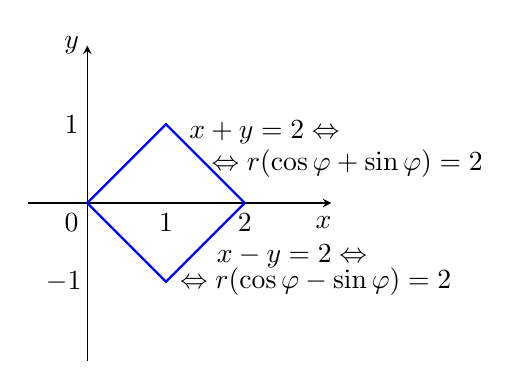
\begin{tikzpicture}[>=stealth]
       % \draw[very thick, blue, fill=pink]
        %(-3,0) -- (-1,0) -- (0,1) -- (1,0) -- (3,0) -- (0,3) -- cycle;
        %\draw[very thick, blue, fill=magenta]
        %(-3,0) -- (-1,0) -- (-0.5,0.5) -- (-0.5,2.5) -- cycle;
        \draw[->] (-0.75,0) -- (3.1,0); % Ох
        \draw[->] (0,-2) -- (0,2); % Оу
        \node at (-0.2,-0.25) {\color{black} $0$};
        \node at (3,-0.25) {\color{black} $x$};
        \node at (-0.2,2) {\color{black} $y$};
        \node at (1,-0.25) {\color{black} $1$};
        \node at (2,-0.25) {\color{black} $2$};
        \node at (-0.2,1) {\color{black} $1$};
        \node at (-0.3,-1) {\color{black} $-1$};
        \node at (2.25,0.9) {\color{black} $x+y=2 \Leftrightarrow$};
        \node at (3.3,0.5) {\color{black} $\Leftrightarrow r (\cos \varphi+\sin \varphi)=2$};
        \node at (2.6,-0.67) {\color{black} $x-y=2 \Leftrightarrow$};
        \node at (2.9,-1) {\color{black} $\Leftrightarrow r (\cos \varphi-\sin \varphi)=2$};
        \draw[thick, blue, domain=0:2] plot (\x, {abs(\x-1)-1});
        \draw[thick, blue, domain=0:2] plot (\x, {1-abs(\x-1)});
    \end{tikzpicture}
    \end{wrapfigure}
    \begin{flalign*}
        & |x-1| + |y| \le 1 \\[5 pt]
        & \text{Область представляет собой ромб с центром в точке $(1, 0)$} \\
        & \text{Из рисунка видно, что угол $\varphi$ лежит в пределах $\left[-\pi/4; \pi/4\right]$} \\
        & \text{Можно определить и отрезки для $r$}: \\
        & r \in \left\{\begin{array}{ll} 
            \left[ 0; \dfrac2{\cos \varphi + \sin \varphi} \right], & \varphi \ge 0 \\[10 pt]
            \left[ 0; \dfrac2{\cos \varphi - \sin \varphi} \right], & \varphi < 0  \\ 
        \end{array}\right. \\
        & \iint\limits_D f(r \cos \varphi, r \sin \varphi\, d\varphi\,dr
        = \int\limits_{-\pi/4}^{0} d\varphi \int\limits_{0}^{\frac2{\cos \varphi - \sin \varphi}} f(r \cos \varphi, r \sin \varphi)\, r \,dr + \int\limits_{0}^{\pi/4} d\varphi \int\limits_{0}^{\frac2{\cos \varphi + \sin \varphi}} f(r \cos \varphi, r \sin \varphi)\, r \,dr = \\[-10 pt]
        & = \int\limits_{-\pi/4}^{\pi/4} d\varphi \int\limits_{0}^{\frac2{\cos \varphi + |\sin \varphi|}} f(r \cos \varphi, r \sin \varphi)\, r \,dr \\
        & \text{При $r \in [0; \sqrt2]$ все углы от $-\pi/4$ до $\pi/4$ лежит в нужной области} \\[-5 pt]
        & \text{При $r \in (\sqrt2; 2 \sqrt2]$ необходимо } 2 \ge r (\cos \varphi + |\sin \varphi|) \\
        & \text{Так как относительно $Oy$ все симметрично, найдем границу при $\varphi > 0$:} \\
        & \text{из геометрии рисунка (треугольников и всего такого)} \\[-10 pt]
        & r \cos \left( \dfrac{\pi}4 - \varphi \right) = \sqrt2 
        \Leftrightarrow \cos \left( \dfrac{\pi}4 - \varphi \right) = \dfrac{\sqrt2}r
        \Leftrightarrow \varphi = \frac{\pi}4 - \arccos \dfrac{\sqrt2}{r} \\[-5 pt]
        & \text{Повторный интеграл с найденными границами:} \\[-10 pt]
        & \int\limits_{0}^{\sqrt2} r\, dr \int\limits_{-\pi/4}^{\pi/4} f(r \cos \varphi, r \sin \varphi)\, d\varphi 
        + \int\limits_{\sqrt2}^{2\sqrt2} r\, dr \int\limits_{\arccos \frac{\sqrt2}{r} - \frac{\pi}4}^{\frac{\pi}4 - \arccos \frac{r}{\sqrt2}} f(r \cos \varphi, r \sin \varphi)\, d\varphi 
    \end{flalign*}
    
    \subsection*{Задача 5}
    
    $D$ -- множество, лежащее в круге $x^2 + y^2 \leq 1$ вне кривой $r = \cos 3 \varphi.$
    
    
    Для начала простое. $x^2 + y^2 \leq \iff r \leq 1 \implies r \in [0,1].$
    
    Теперь разберёмся с кривой $r  = \cos 3 \varphi$.
    
    Если $r \in [0,1], \; $ то $\cos 3 \varphi \in [0,1] \implies 3 \varphi \in \left[ -\frac{\pi}{2} + 2\pi n, \frac{\pi}{2} + 2\pi n \right].$
    
    \doublespacing $\begin{cases}
    n = 0 \; \to \; \varphi \in \left[ -\frac{\pi}{6},  \frac{\pi}{6} \right];\\
    n = 1\; \to \; \left[\frac{\pi}{2},  \frac{5\pi}{6} \right]; \\
    n = 2\; \to \;  \left[ \frac{7\pi}{6},  \frac{3\pi}{2} \right]. \\
    \end{cases}$
    
    Т.е. $\varphi \in  \left[ -\frac{\pi}{6},  \frac{\pi}{6} \right] \cup \left[\frac{\pi}{2},  \frac{5\pi}{6} \right]\cup \left[ \frac{7\pi}{6},  \frac{3\pi}{2} \right].$
    
    [picture is coming soon]
    
    \singlespacing Мы готовы записать интеграл, не забываем указывать якобиан!
    
    $\boxed{ \displaystyle \int\limits_{-\pi/6}^{\pi/6} d \varphi \int\limits_{\cos 3 \varphi}^{1} r \cdot f \; dr + \int\limits_{\pi/2}^{5\pi/6} d \varphi \int\limits_{\cos 3 \varphi}^{1} r \cdot f \; dr + 
    \int\limits_{7\pi/6}^{3\pi/2} d \varphi \int\limits_{\cos 3 \varphi}^{1} r \cdot f \; dr} \; $
    
    
    \subsection*{Задача 6}
    $D$ --- множество, лежащее вне окружности $x^2 + y^2 = 1$ и внутри петель кривой $(x^2 + y^2)^2 = 2(x^2 - y^2)$ \\[5 pt]
    Так как область лежит вне окружности $x^2 + y^2 = 1$, в полярных координатах $r > 1$. \\[3 pt]
    Определим условия, необходимые и достаточные для того, чтобы координаты лежали внутри петель кривой: \\[3 pt]
    $(x^2 + y^2)^2 = 2\, (x^2 - y^2) \Leftrightarrow r^4 = 2\, r^2 (\cos^2 \varphi - \sin^2 \varphi)
     \Leftrightarrow r^2 = 2 \cos 2\, \varphi$ \\[5 pt]
     Тогда точка с полярными координатами $(r, \varphi)$ лежит внутри петель, если 
     $r^2 \le 2 \cos 2\, \varphi \Leftrightarrow \cos 2\, \varphi \ge \dfrac{r^2}2 \Leftrightarrow 
     \varphi \in \left[ -\dfrac12\arccos \dfrac{r^2}2; \dfrac12\arccos \dfrac{r^2}2 \right]$ \\
     Повторный интеграл:
     $\int\limits_{1}^{\sqrt2} r\, dr \int\limits_{-\frac12\arccos \frac{r^2}2}^{\frac12\arccos \frac{r^2}2} f(r \cos \varphi, r \sin \varphi)\, d\varphi$
    
    \section*{Перейдя к полярным координатам, вычислите интеграл.}
    \subsection*{Задача 7}
    
    $\displaystyle \iint\limits_{D} \ln (1 + x^2 + y^2) dx dy, \; \, D = \{(x,y) \mid x^2 + y^2 \leq 4 \} .$
    
    $D$ -- круг с радиусом $2 \implies r \in [0,2]$.
    
    $\varphi \in [0, 2 \pi),$ как и всегда.
    
    $\displaystyle \int\limits_{0}^{2} dr \int\limits_{0}^{2 \pi} r \cdot \ln(1 + r^2) d \varphi = \int\limits_{0}^{2} 2 \pi \cdot r \cdot \ln(1 + r^2) dr =  \pi \int\limits_{0}^{2} 2  \cdot r \cdot \ln(1 + r^2) dr.$
    
    Замена $\begin{cases} t = 1 + r^2;\\
    dt = 2r \, dr;\\
    r \in [0, 2] \implies t \in [1,5] \end{cases}$
    
    $\dots = \pi \int\limits_{1}^{5} \ln (t) \, dt = \pi \cdot \left(  t \ln t - t \, \Bigg|_{1}^{5} \right) = \pi \cdot \left( 5 \ln 5 - 5 + 1\right) = \boxed{ \pi (5 \ln 5 - 4) } 
    \; .$
    
    \subsection*{Задача 8}
    \begin{flalign*}
        & \iint\limits_D \frac{x dxdy}{\sqrt{4 - x^2 - y^2}}, \;\; D = \left\{ (x, y) | x^2 + y^2 \leq 2x \right\} \\
        & \begin{cases} 
            x = r \cos \varphi \\
            y = r \sin \varphi 
        \end{cases} \Rightarrow D = \left\{ (r, \varphi) | r \leq 2 \cos \varphi \right\} \\
        & \iint\limits_D \frac{r \cos \varphi}{\sqrt{4 - r^2}} r d \varphi d r = 
        \int\limits_{0}^{2} dr \int\limits_{-\arccos \left( r/2 \right)}^{\arccos \left( r/2 \right)} 
        \frac{r^2 \cos \varphi}{\sqrt{4 - r^2}} d \varphi = 
        \int\limits_{0}^{2} \frac{r^2}{\sqrt{4 - r^2}} dr 
        \int\limits_{-\arccos \left( r/2 \right)}^{\arccos \left( r/2 \right)} 
        \cos \varphi d \varphi = \\
        & = \int\limits_{0}^{2} \frac{r^2}{\sqrt{4 - r^2}} dr 
        \left. \sin \varphi \right|_{-\arccos \left( r/2 \right)}^{\arccos \left( r/2 \right)} = 
        \int\limits_{0}^{2} \frac{r^2}{\sqrt{4 - r^2}} \sqrt{4 - r^2} dr = \int_0^2 r^2 dr = \frac{8}{3}
    \end{flalign*}
    
    \section*{Перейдите к переменным, в которых область интегрирования имеет вид прямоугольника, 
    и вычислите интеграл.}
    
    \subsection*{Задача 9}
    
    $\displaystyle\iint\limits_{D} \frac{(x + y)^2}{x} dx dy; \; \, D = \{(x,y) \mid 1 - x \leq y \leq 3 - x, \; \; \frac{x}{2} \leq y \leq 2x \}.$
    
    Область интегрирования имеет вид прямоугольника -- значит, нам нужно, чтобы граница каждого интеграла изменялась от одной константы до другой константы.
    
\doublespacing    $\begin{cases} u := x + y \implies 1 \leq u \leq 3 \text{ из 1-го нер-ва.} \\
    v := \frac{y}{x} \implies \frac{1}{2} \leq v \leq 2 \text{ из 2-го нер-ва. }
    \end{cases}$
    
    \singlespacing Т.е. с помощью подобной замены мы смогли выполнить поставленную задачу (обе координаты ограничены только константами и не зависят друг от друга).  
    
    Выражаем теперь, обратно, $x$ и $y$ через $u$ и $v$.
    
    $x = u - y.$
    
    $\begin{cases}
    y = v \cdot x = v \cdot (u - y)  = v \cdot u - v \cdot y \implies y = \frac{v \cdot u}{1 + v}; \\
    x = u - \frac{v \cdot u}{1 + v} = \frac{u + uv - uv}{1 + v} = \frac{u}{1 + v} . \end{cases}$
    
    Считаем якобиан. Для удобства взятия производной, лучше игрек перепишем как $y = \frac{v \cdot u}{1 + v} = u - \frac{u}{1 + v}.$
    
     
    $J = \left| \begin{matrix} x_u & y_u \\ x_v & y_v \end{matrix} \right| = $ {\setstretch{2.4} $
     \left| \begin{matrix} \left(\frac{u}{1 + v}\right)_u & \left(u - \frac{u}{1 + v}\right)_u \\ \left(\frac{u}{1 + v}\right)_v & \left(u - \frac{u}{1 + v} \right)_v \end{matrix} \right| =  
     \left| \begin{matrix} \frac{1}{1 + v} & \frac{v}{1 + v} \\ \frac{-u}{(1 + v)^2} & \frac{u}{(1 + v)^2} \end{matrix} \right| $} = $\frac{u}{(1 + v)^3} + \frac{uv}{(1 + v)^3} = \frac{u(1 + v)}{(1 + v)^3} = \frac{u}{(1 + v)^2} \; .$
     
     Теперь перепишем функцию в новых координатах.
     
     $f = \frac{(x + y)^2}{x} = \frac{u^2}{u/(1 + v)} = u(1 + v).$
    
     Всё, теперь мы готовы брать интеграл.
     
     $\displaystyle \int\limits_{1/2}^{2} dv \int\limits_{1}^{3} (1 + v) \cdot u \cdot \left| \frac{u}{(1 + v)^2} \right| \, du = [\text{помним, что } u \text{ -- положительный}] = \int\limits_{1/2}^{2} \frac{1}{1 + v} \int\limits_{1}^{3} u^2 \, du = 
     \int\limits_{1/2}^{2} \frac{1}{1 + v} \cdot  \left(\frac{u^3}{3} \; \;  \Bigg|_{1}^{3} \right) = \\
     = \int\limits_{1/2}^{2} \frac{1}{1 + v} \cdot \frac{26}{3} dv = \frac{26}{3} \; \int\limits_{1/2}^{2} \frac{1}{1 + v}dv. $
     
     Замена $\begin{cases} t = 1 + v;\\
     dt  = dv;\\
     v \in [1/2, \; 2] \implies t \in [3/2, \; 3]
     \end{cases}$
     
     $\dots = \frac{26}{3} \int \limits_{3/2}^{3} \frac{1}{t} = \frac{26}{3} \left( \ln t \;  \Bigg|_{3/2}^{3} \right) = \frac{26}{3} \cdot (\ln 3 - \ln (3/2)) = \boxed{\frac{26}{3} \ln 2 } \; .$
     
    
    \subsection*{Задача 10}
    \begin{flalign*}
        & \iint\limits_D xy(x+y) dxdy, \;\;\;\;\;\; D = \left\{ (x, y) \Big| -1 \leq x - y \leq 1, 
        \frac{1}{x} \leq y \leq \frac{2}{x} \right\} \\
        & \begin{cases} 
            u = x - y & u \in [-1, 1]\\
            v = xy & v \in [1, 2]
        \end{cases} \Rightarrow x = u + y \Rightarrow v = uy + y^2 \Rightarrow y = \frac{-u \pm \sqrt{u^2 + 4v}}{2} \\
        & u^2 + 4v \geq 4 \Rightarrow \sqrt{u^2 + 4v} \geq 2 \Rightarrow y_{-} \leq \frac{-u - 2}{2} \Rightarrow y_{-} < 0.
        \text{ По картинке } y > 0 \Rightarrow y = y_{+} = \frac{-u + \sqrt{u^2 + 4v}}{2} \\
        & x = u + y = u + \frac{-u + \sqrt{u^2 + 4v}}{2} = \frac{u + \sqrt{u^2 + 4v}}{2} \\
        & \begin{cases} 
            x = \frac{u + \sqrt{u^2 + 4v}}{2} \\
            y = \frac{-u + \sqrt{u^2 + 4v}}{2}  
        \end{cases} \Rightarrow J = \begin{pmatrix}
            \frac{1}{2} + \frac{u}{2\sqrt{u^2 + 4v}} & \frac{1}{\sqrt{u^2 + 4v}} \\
            - \frac{1}{2} + \frac{u}{2\sqrt{u^2 + 4v}} & \frac{1}{\sqrt{u^2 + 4v}} \\
        \end{pmatrix} \;\;\;\;\;\; |J| = \frac{1}{\sqrt{u^2 + 4v}} \\
        & \int\limits_{-1}^1 du \int\limits_1^2 
        v \left( \frac{u + \sqrt{u^2 + 4v}}{2} + \frac{-u + \sqrt{u^2 + 4v}}{2} \right) |J| dv = 
        \int\limits_{-1}^1 du \int\limits_1^2 v \frac{\sqrt{u^2 + 4v}}{\sqrt{u^2 + 4v}} dv = 
        \int\limits_{-1}^1 du \int\limits_1^2 v dv = 3
    \end{flalign*}

    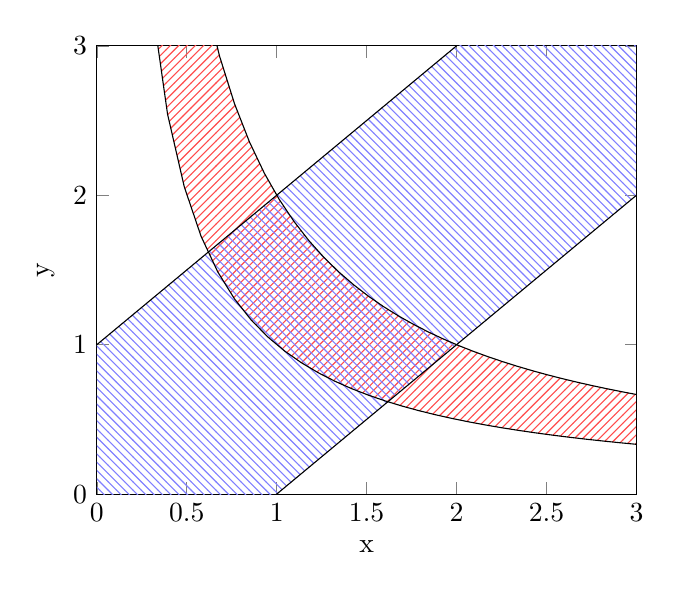
\begin{tikzpicture} 
        \begin{axis}[xmin=0, xmax=3, ymin=0, ymax=3, xlabel=x, ylabel=y]
            \addplot[domain=0.3:3, samples=30, variable=\x, name path=A] ({\x}, {1/\x});
            \addplot[domain=0.6:3, samples=30, variable=\x, name path=B] ({\x}, {2/\x});
            \addplot[pattern color=red!70, pattern=north east lines] fill between [of=A and B];
            \addplot[domain=0:3, name path=C] {x+1};
            \addplot[domain=0:3, name path=D] {x-1};
            \addplot[pattern color=blue!50, pattern=north west lines] fill between [of=C and D];
        \end{axis} 
    \end{tikzpicture}   
    
    \subsection*{Задача 11}
    
    $\displaystyle \iint\limits_{D} xy \;  dxdy; \; \; D = \{(x,y) \mid x^3 \leq y \leq 2 x^3, \; 2x \leq y^2 \leq 3x\}.$
    
    { \setstretch{2} $\begin{cases}u = \frac{y}{x^3} \implies 1 \leq u \leq 2; \\
    v = \frac{y^2}{x} \implies 2 \leq v \leq 3
    \end{cases}$}
    
    Выражаем $x$ и $y$:
    
    $x = \frac{y^2}{v}.$\\
    
    $\begin{cases}
    y = x^3 \cdot u = \frac{y^6}{v^3} \cdot u \implies \frac{1}{y^5} = \frac{u}{v^3} \implies y = \sqrt[5]{ \frac{v^3}{u}} = v^{3/5} \cdot u^{-1/5};\\
    x = \frac{y^2}{v} =  v^{6/5} \cdot u^{-2/5} \cdot v^{-1} = v^{1/5} \cdot u^{-2/5}
    \end{cases}$
    
    
    Перепишем функцию:
    
    $f = xy = v^{3/5} \cdot v^{1/5} \cdot u^{-1/5} \cdot u^{-2/5}  = v^{4/5} \cdot u^{-3/5}.$
    
    
    Ищем якобиан.
    
     $J = \left| \begin{matrix} x_u & y_u \\ x_v & y_v \end{matrix} \right| = $ {\setstretch{2} $
     \left| \begin{matrix} \left(v^{1/5} \cdot u^{-2/5}\right)_u & \left(v^{3/5} \cdot u^{-1/5} \right)_u \\ \left(v^{1/5} \cdot u^{-2/5} \right)_v & \left(v^{3/5} \cdot u^{-1/5}  \right)_v \end{matrix} \right| =  
     \left| \begin{matrix}   -2/5 \cdot v^{1/5} \cdot u^{-7/5} & -1/5 \cdot v^{3/5} \cdot u^{-6/5}\\ 
     1/5 \cdot v^{-4/5} \cdot u^{-2/5} & 3/5 \cdot v^{-2/5} \cdot u^{-1/5}\\   \end{matrix} \right| $} = \\ $-\frac{6}{25} v^{-1/5} \cdot u^{-8/5} + 
     \frac{1}{25} v^{-1/5} \cdot u^{-8/5} = - \frac{v^{-1/5} \cdot u^{-8/5}}{5}.$
     
     Всё готово для подсчёта интеграла. Заметим, что $J < 0 \implies |J| = -J.$
     
     $I = \displaystyle \int \limits_{1}^{2} du \int \limits_{2}^{3} v^{4/5} \cdot u^{-3/5} \cdot |J| \;  dv = \frac{1}{5} \int\limits_{1}^{2} du \int \limits_{2}^{3} v^{4/5} \cdot u^{-3/5} \cdot v^{-1/5} \cdot u^{-8/5} \; dv= 
     \frac{1}{5} \int\limits_{1}^{2} du \int \limits_{2}^{3} v^{3/5} \cdot u^{-11/5} \; dv = \\ 
     = \frac{1}{5} \int\limits_{1}^{2} u^{-11/5} \; du \left(\frac{8}{5} \cdot v^{5/8} \;  \Bigg|_{2}^{3} \right) = \frac{1}{8} \cdot  (3^{8/5} - 2^{8/5}) \cdot \int\limits_{1}^{2} u^{-11/5} \; du =  
     \frac{1}{8} \cdot  (3^{8/5} - 2^{8/5}) \cdot \left( -\frac{5}{6} u^{-6/5}
     \; \, \Bigg|_{1}^{2} \right)\; du = \\ \boxed{\frac{5}{46} \cdot (3^{8/5} - 2^{8/5}) \cdot (1 - 2^{-6/5})} \; .$
    
    
    
    \subsection*{Задача 12}
    \begin{wrapfigure}{r}{0.4\textwidth}
    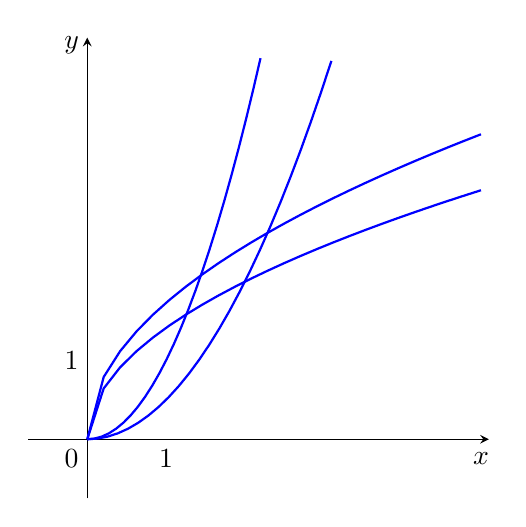
\begin{tikzpicture}[>=stealth]
        \draw[->] (-0.75,0) -- (5.1,0); % Ох
        \draw[->] (0,-0.75) -- (0,5.1); % Оу
        \node at (-0.2,-0.25) {\color{black} $0$};
        \node at (5,-0.25) {\color{black} $x$};
        \node at (-0.2,5) {\color{black} $y$};
        \node at (1,-0.25) {\color{black} $1$};
        % \node at (2,-0.25) {\color{black} $2$};
        \node at (-0.2,1) {\color{black} $1$};
        % \node at (2.25,0.9) {\color{black} $x+y=2 \Leftrightarrow$};
        % \node at (3.3,0.5) {\color{black} $\Leftrightarrow r (\cos \varphi+\sin \varphi)=2$};
        % \node at (2.6,-0.67) {\color{black} $x-y=2 \Leftrightarrow$};
        % \node at (2.9,-1) {\color{black} $\Leftrightarrow r (\cos \varphi-\sin \varphi)=2$};
        \draw[thick, blue, domain=0:2.2] plot (\x, {\x*\x});
        \draw[thick, blue, domain=0:3.1] plot (\x, {0.5*\x*\x});
        \draw[thick, blue, domain=0:5] plot (\x, {sqrt(2*\x)});
        \draw[thick, blue, domain=0:5] plot (\x, {sqrt(3*\x)});
    \end{tikzpicture}
    \end{wrapfigure}
    \begin{flalign*}
        & \iint\limits_D \dfrac{x^2 \sin (xy)}{y}\, dx\,dy, \;\;\; D = \{(x, y) \,|\, y \le x^2 \le 2y,\; 2x \le y^2 \le 3x\} \\
        & \text{Хотим, чтобы область, заданная пересечением парабол, была} \\
        & \text{прямоугольником в какой-то системе координат} \\
        & \text{Перейдем к координатам $u$ и $v$ таким, что } u = \dfrac{x^2}y, \; v = \dfrac{y^2}x. \\
        & \text{Тогда } D = \{ (u, v) \,|\, 1 \le u \le 2, \; 2 \le v \le 3 \} \\[5 pt]
        & \text{Выражение старых координат через новые:} \\[-5 pt]
        & u = \dfrac{x^2}y \Rightarrow y = \dfrac{x^2}u \Rightarrow v = \dfrac{x^4}{u^2 x} = \dfrac{x^3}{u^2}
        \Rightarrow x = \sqrt[3]{u^2 v}, \; y = \sqrt[3]{\dfrac{u^4 v^2}{u^3}} = \sqrt[3]{u v^2} \\
        & J = \left|\begin{matrix} x_u & y_u \\ x_v & y_v \end{matrix}\right| = 
        \left|\begin{matrix} \dfrac23 \sqrt[3]{\dfrac{v}{u}} & \dfrac13\sqrt[3]{\dfrac{v^2}{u^2}} \\[10 pt] \dfrac13\sqrt[3]{\dfrac{u^2}{v^2}} & \dfrac23\sqrt[3]{\dfrac{u}{v}} \end{matrix}\right| = \dfrac49\sqrt[3]{\dfrac{uv}{uv}} - \dfrac19\sqrt[3]{\dfrac{u^2v^2}{u^2v^2}} = \dfrac{4}{9} - \dfrac{1}{9} = \dfrac13 \\
        & I = \int\limits_1^2 du \int\limits_2^3 \dfrac{\sqrt[3]{u^4 v^2} \sin (uv)}{\sqrt[3]{uv^2}} \cdot \dfrac13\, dv = 
        \dfrac13 \int\limits_1^2 u\, du \int\limits_2^3 \sin (uv)\, dv = \\ 
        & = \dfrac13 \int\limits_1^2 u\, du \left( -\dfrac1u\, \cos(uv) \right) \Bigm|_2^3 
        = \dfrac13 \int\limits_1^2 \left( \cos 2u - \cos 3u \right)\, du -\dfrac1u\, \cos(uv) \Bigm|_2^3 = \\
        & = \dfrac13  \left( \dfrac12\, \sin 2u - \dfrac13\, \sin 3u \right) \Bigm|_1^2 
        = \dfrac13 \left( \dfrac12 \left( \sin4 - \sin2 \right) - \dfrac13 \left( \sin6 -\sin3 \right) \right)
    \end{flalign*}
    
    \section*{Задайте в цилиндрических координатах множество $D$, заданное неравенствами в декартовых
    координатах. Пердполагаю функцию $f$ непрерывной на $D$, преобразуйте интеграл в цилиндрических
    координатах к повторному.}
    
    \subsection*{Задача 13}
    
    $x^2 + y^2 \leq 1, \; x^2 + y^2 + z^2 \leq 4.$
    
    $\bullet \; $ Первое неравенство:
    
    $r^2 \leq 1 \implies r \in [0,1].$
    
    $\bullet \; $ Второе неравенство:
    
    $r^2 + z^2 \leq 4 \implies |z| \leq \sqrt{4 - r^2} \implies z \in [-\sqrt{4 - r^2}, \; \sqrt{4 - r^2}].$
    
    Ограничений на  $\varphi$ никаких нет. Можем приступать к записи интеграла. Помним, что в циллиндрических координатах $|J| = r.$
    
    $I = \boxed{\displaystyle \int\limits_{0}^{2 \pi} d \varphi \int\limits_{0}^{1} dr \int\limits_{-\sqrt{4 - r^2}}^{\sqrt{4 - r^2}} f(r \cos \varphi, \; r \sin \varphi, z) \cdot r \; dz} \; .$
    
     
    \subsection*{Задача 14}
    
    $x^2 + y^2 + z^2 \leq  2z, \; x^2 + y^2 \leq z^2.$
    
    $\bullet$ Первое нер-во.
    
    $x^2 + y^2 \leq 2z - z^2 \iff r^2 \leq 2z-z^2.$ 
    
    Значит, значение $2z - z^2$ обязано быть положительным. Парабола с нулями в 0 и 2 $\implies z \in [0, \, 2].$
    
    В таком случае $r \in \left[0, \; \sqrt{2z - z^2} \right].$
    
    $\bullet$ Второе нер-во.
    
    $r^2 \leq z^2 \implies r \in \left[0, \, |z|\right].$ Так как $z \geq 0$, то $|z| = z.$ 
    
    Заметим, что при $z \in [0, \, 2]$ всегда выполнено $2 \geq z \iff 2z \geq 2z^2 \iff \sqrt{2z - z^2} \geq z .$
    
    Так что границы $r$ переписываем полностью как $r \in [0,z].$
    
    На $\varphi$ ограничений нет, модуль якобиана равен $r$.
    
    $\boxed{\displaystyle \int\limits_{0}^{2 \pi} d \varphi \int\limits_{0}^{2} dz \int\limits_{0}^{z} f \cdot r \; dr} \; .$
    
    \section*{Перейдя к цилиндрическим координатам, вычислите интеграл.}
    \subsection*{Задача 15}
    \begin{flalign*}
        & \iiint\limits_D z dxdydz \;\;\;\;\;\; D = \left\{ (x, y, z) | x^2 + y^2 \leq z^2, \; 0 \leq z \leq 1 \right\} 
        \Rightarrow D = \left\{ (r, \varphi, z) | r^2 \leq z^2, \; 0 \leq z \leq 1 \right\} \\
        & \int_{0}^{2\pi} d\varphi \int_0^1 z  dz \int_0^z r dr = 
        \int_{0}^{2\pi} d\varphi \int_0^1 z \frac{z^2}{2} dz = 
        2 \pi \frac{1}{8} = \frac{\pi}{4} 
    \end{flalign*}
    
     \subsection*{Задача 16}
     
     $\displaystyle \iiint_{D} z^2 \; dxdydz, \; \; D = \{(x,y,z) \mid x^2 + y^2 + z^2 \geq 1, \; x^2 + y^2 + z^2 \leq 2z\}.$
     
     $\bullet$ Первое нер-во.
     
     $x^2 + y^2 + z^2 \geq 1 \iff r^2 \geq 1 \implies r \geq 1.$
     
     $\bullet$ Второе нер-во.
     
     $x^2 + y^2 + z^2 \leq 2z \implies$ как в номере $14$, $z \in [0,2];\; \, r \leq z.$
     
     По $\varphi$ область не ограничена. Модуль якобиана равен $r$. Сразу вынесу все константы за интегралы:
     
     
     $\displaystyle \int\limits_{0}^{2} z^2 \; dz  \int\limits_{0}^{z} r \; dr  \int\limits_{0}^{2 \pi} 1\;  d \varphi = 2 \pi \cdot
     \int\limits_{0}^{2} z^2 \; dz  \; \left( \frac{r^2}{2} \; \Bigg|_{0}^{z}  \right) = \pi \cdot \int\limits_{0}^{2} z^4 \; dz = \\ 
     \pi \cdot \left( \frac{z^5}{5} \;  \Bigg|_{0}^{2}\right) = \boxed{\frac{32 \pi}{5}} \; . $
    
    \section*{Задайте в сферических координатах множество $D$, заданное неравенствами в декартовых координатах.
    Предполагая функцию $f$ непрерывной на $D$, преобразуйте интеграл в сферических координатах к повторному.}
    
    
    \subsection*{Задача 17}
    
    $x^2 + y^2 + z^2 \leq 1; \; x^2 + y^2 + z^2 \leq 2z.$
    
    \underline{Используем следующую замену:}
    
    $\begin{cases}
    x = r \cos \varphi \sin \Theta;\\
    y = r \sin \varphi \sin \Theta;\\
    z = r  \cos \Theta;\\
    \end{cases}$
    
    $\bullet \; $ Первое неравенство:
    
    $x^2 + y^2 + z^2 \leq 1 \implies r^2 \leq 1 \implies r \in [0,1].$
    
    $\bullet \; $ Второе неравенство:
    
    $x^2 + y^2 + z^2 \leq 2z \iff r^2 \leq 2 r \cos \Theta \iff r \leq 2 \cos \Theta.$
    
    Заметим, что при этих ограничениях: $\; \; \begin{cases} 
    2 \cos \Theta > 1 \implies r \in [0,1];\\
    2 \cos \Theta \leq 1 \implies r \in [0, 2 \cos \Theta]
    \end{cases} \iff 
    \begin{cases} 
    r \in [0,1], \; \, \Theta \in \left[\frac{\pi}{3}, \; \pi \right];\\
    r \in \left[0, 2 \cos \Theta \right], \; \, \Theta \in \left[0, \; \frac{\pi}{3} \right)
    \end{cases}$
    
    $\varphi$ остаётся без ограничений.
    
    Якобиан в сферических координатах (при данной! замене) равен $r^2 \sin \Theta.$
    
    Итог:
    
    $\boxed{\displaystyle \int\limits_{0 }^{2 \pi} d \varphi\left( 
    \int\limits_{0 }^{\pi/3} d \Theta \int\limits_{0 }^{2 \cos \Theta} f \cdot r^2 \sin \Theta \; dr + 
    \int\limits_{\pi/3 }^{\pi} d \Theta \int\limits_{0 }^{1} f \cdot r^2 \sin \Theta \; dr
    \right) } \; .$
    
    
    
    
    \subsection*{Задача 18}
    
    $x^2 + y^2 + z^2 \leq 2y, \; x^2 + y^2 \geq z^2.$
    
    
    $\bullet$  Первое нер-во.
    
    \onehalfspacing $x^2 + y^2 + z^2 \leq 2y \iff r^2 \leq 2 \, r \sin \varphi \sin \Theta \iff r \leq 2 \sin \varphi \sin \Theta \implies r \in [0, 2 \sin \varphi \sin \Theta].$
    
    \singlespacing Также мы должны учесть, что $\sin{\varphi}$ обязан быть неотрицательным, ведь $r \geq 0 \land \sin \Theta \geq 0.$
    
    То есть $\varphi \in [0, \pi].$
    
    $\bullet$  Второе нер-во.
    
    $x^2 + y^2 \geq z^2 \iff r^2 \sin^2 \Theta \geq r^2 \cos^2 \Theta \implies \tg^2 \Theta \geq 1 \implies |\tg \Theta| \geq 1.$
    
    Значит, $\Theta \in \left[ \frac{\pi}{4}, \; \frac{3\pi}{4} \right].$
    
    Модуль Якобиана в сферических координатах с данной заменой -- $r^2 \sin \Theta.$
    
    Всё готово, выписываем интеграл.
    
    $\boxed{\displaystyle
    \int \limits_{\pi/4}^{3 \pi /4} d \Theta \int \limits_{0}^{\pi} d \varphi \int \limits_{0}^{2 \sin \varphi \sin \Theta} f \cdot r^2 \sin \Theta \; dr} \; .$
    
    \section*{Перейдя к сферическим координатам, вычислите интеграл.}
    
    
    \subsection*{Задача 19}
    
    $\displaystyle \iiint\limits_{D} (x^2 + y^2 + z^2) \; dx \, dy\, dz; \; D = \{(x,y,z) \mid x^2 + y^2 + z^2 \leq 1, \; y^2 + z^2 \leq x^2, \; x \geq 0 \}. $
    
    [picture is coming soon]
    
    \underline{Лайфхак}: если мы видим, что с какой-то координатой возникают потенциальные трудности, делаем её в качестве оси, отвечающей за "широту". В данной ситуации нам подойдёт следующая замена:
    
    $\begin{cases}
    x = r \cos \Theta;\\
    y = r \sin  \varphi \sin  \Theta;\\
    z = r \cos  \varphi \sin  \Theta \\
    \end{cases} \; \; \; \; 
    \begin{cases}
    \Theta \in [0,\pi];\\
    \varphi \in [0, 2 \pi)
    \end{cases}$
    
    $\bullet$ Первое неравенство.
    
    $x^2 + y^2 + z^2 \leq 1 \implies r^2 \leq 1 \implies r \in [0,1].$
    
    $\bullet$ Третье неравенство.
    
    $x \geq 0 \implies r \cos \Theta \geq 0 \implies \cos \Theta \geq 0 \implies \Theta \in \left[0, \frac{\pi}{2}\right]. $
    
    (Мы использовали тот факт, что $r \geq 0$).
    
    $\bullet$ Второе неравенство.
    
    $y^2 + z^2 \leq x^2 \iff
    r^2 \sin^2  \varphi \cdot \sin^2  \Theta +
    r^2 \cos^2  \varphi \cdot  \sin^2  \Theta \leq 
    r^2 \cos^2 \Theta \implies r^2 \sin^2 \Theta \leq r^2 \cos^2 \Theta \iff \tg^2 \Theta \leq 1 \implies \Theta \in \left[ 0, \frac{\pi}{4} \right].$
    
    На $\varphi$ ограничений нет. $|J| = r^2 \sin \Theta,$ как и при обычной сферической замене.
    
    Интегрируем:
    
    $\displaystyle \int \limits_{0}^{\pi /4} d\Theta  \int \limits_{0}^{1} dr  \int \limits_{0}^{2 \pi}   r^2 \cdot r^2 \sin \Theta \; d \varphi  = 2 \pi \int \limits_{0}^{\pi /4} \sin \Theta \;  d\Theta  \int \limits_{0}^{1}  r^4   \; dr = 2 \pi \cdot  \left( -\cos \Theta \;  \Bigg|_{0}^{\pi /4} \right) \cdot \left( \frac{r^5}{5} \; \Bigg|_0^1 \right) = \boxed{\frac{2\pi}{5} \cdot \left(1 - \frac{1}{\sqrt{2}} \right)} \; .$
    
    
    
    
    \subsection*{Задача 20}
    
    $\iint_{D} z \; dxdydz, \; \; D = \left\{(x,y,z) \, \Big| \;  \frac{x^2}{4} + \frac{y^2 }{9} + z^2 \leq 1, \; z \geq 0 \right\} $
    
    Сначала сделаю финт ушами, и заменю:
    
    $
    \begin{cases}
    x = 2 u;\\
    y = 3 v;\\
    z = w\\
    \end{cases}
    $
    
    Ищем якобиан,
    
    $J =  \left| \begin{matrix} x_u & y_u & z_u \\ x_v & y_v & z_v \\  x_w & y_w & z_w  \end{matrix} \right| = 
      \left| \begin{matrix} 2 & 0 & 0 \\ 0 & 3 & 0 \\  0 & 0 & 1  \end{matrix} \right| = 6.$
    
    Т.е. множитель $6$ мы добавим под интеграл в дальнейшем.
    
    Теперь производим привычную замену на сферические координаты:
    
    
    $\begin{cases}
    u = r \cos \varphi \sin \Theta;\\
    v = r \sin \varphi \sin \Theta;\\
    w = r  \cos \Theta\\
    \end{cases}$
    
    $|J| = r^2 \sin \Theta$, это наряду с 6 появится под интегралом.
    
    Теперь перепишем неравенства.
    
    $\bullet \; \; \frac{x^2}{4} + \frac{y^2}{9} + z^2 \leq 1 \iff \frac{4 u^2}{4} + \frac{9 v^2}{9} + w^2 \leq 1 \iff r^2 \leq 1 \implies  \\ r \in [0, \, 1].$ 
    
    $\bullet \; z \geq 0 \iff w \geq 0 \iff r \; \cos \Theta \geq 0 \implies \cos \Theta \geq 0 \implies \Theta \in \left[0, \frac{\pi}{2}\right].$
    
    $f = z = w = r \cos \Theta.$
    
    Всё, теперь пишем интеграл. На $\varphi$ ограничений нет. Сразу выносим константы.
    
    $\displaystyle \int\limits_{0}^{\pi / 2}  \cos \Theta \; d \Theta \int \limits_{0}^{1} r\;  dr \int\limits_{0}^{2 \pi} 1\;  d \varphi  =  \left( \sin \Theta \; \Bigg|_{0}^{\pi/2}\right) \cdot \left(\frac{r^2}{2} \;  \; \Bigg|_{0}^{1} \right) \cdot 2 \pi= \frac{2 \pi}{2} = \boxed{\pi} \; .$
    
    
    
    
    
    
    
    
    
\end{document}
